\documentclass[]{manual}

\title{Diffraction Gratings}
\date{\today}
\course{Physics 325}

\begin{document}
    \maketitle
    \thispagestyle{firstpage}

    %%%

    \section*{Motivation}

    Light has become one of the primary tools that scientists in nearly every field use to measure the properties of matter.
    Quickly and efficiently determining the wavelength of light is therefore of obvious practical importance.
    A device that does this by separating the wavelengths and projecting them to known positions is called a \textbf{spectrometer}.
    Spectrometers based on \textbf{diffraction gratings} are quite common, and can be delivered in small, robust packages.
    The popularity of these devices means that, in practice, you may never have to use a diffraction grating manually.
    Therefore, the purpose of this lab is to gain both practical and theoretical experience with a diffraction grating.

    \section*{Background}

    The theory of the diffraction grating spectrometer is built on the concepts studied more closely in the slit diffraction lab, where we look at diffraction from a small number of slits.
    A diffraction grating is the result of multi-slit diffraction when the number of slits is so large that the intensity pattern begins to resemble that of multiple-plane-wave interference.
    It is actually somewhat simpler than slit diffraction, although we will need to use a result that will be derived in that lab.
    If a plane wave is normally incident on $N$ slits of width $W$ and spacing $D$, then the optical intensity at a viewing angle $\theta$ is 
    \begin{align}
        I(\theta) = \frac{A_0^2 W^2}{r^2} \mathrm{sinc}^2 \left(\pi W \sin(\theta) / \lambda\right)\frac{\sin^2(\pi N D \sin(\theta) / \lambda)}{\sin^2(\pi D \sin(\theta) / \lambda)}
    \end{align}
    The first term is an unimportant overall scale factor, and the second term is an envelope function determined by the width $W$ of a single slit.
    We will take the limit $W \to 0$ so that this term vanishes (because $\sinc(0) = 1$).
    
    The third term (the ratio of sines) is the most important.
    When $N$ is very large, the amplitude is sharply peaked when the denominator of this ratio is nearly zero.
    This property is precisely what a diffraction grating is based on.

    The positions where the denominator vanishes are called the \textbf{principal maxima}, and they occur when
    \begin{align} \label{eqn:normal-grating-equation}
        \frac{\pi D \sin{\theta}}{\lambda} &= m \pi \nonumber \\
        D \sin{\theta} &= m \lambda.
    \end{align}
    This is the \textbf{grating equation for illumination at normal incidence}.
    The integer $m$ is the \textbf{order}.
    If we shone light composed of many wavelengths on these slits, the output intensity pattern would be a single bright spot for each wavelength of light, for each order.
    Since these occur at different angles, we can use a grating to separate wavelengths of light, in much the same way that a prism does.

    Unfortunately, it turns out that normal incidence isn't particularly useful.
    We need an equation that describes what happens for non-normal incidence.
    To derive a grating equation for non-normal incidence, let's go back to the geometric picture of light incident on an array of thin slits.
    When light is normally incident on a set of slits, the maxima of the interference pattern on the other side will occur when the phase difference between adjacent slits is a multiple of $2 \pi$, or equivalently that the path length difference is a multiple of $\lambda$.
    This is illustrated in Figure~\ref{fig:path-length-difference-normal}.

    \begin{figure}[H]
        \centering

        \begin{tikzpicture}
        \foreach \y in {0, 1, 2, 3, 4} {
            \draw[very thick] (0, \y + .1) -- (0, \y + .9);
        }

        \foreach \y in {1, 2, 3, 4} {
            \draw[midarrow = {stealth}] (0, \y) -- ++(20:2);
            \draw[revmidarrow = {stealth}] (0, \y) -- ++(180:2);
            \draw[dotted, thick] (0, \y) -- ++ (-70:{(\y-1) * sin(70)});
        }

        \draw[dashed] (0, 1) -- (-2, 1);
        \draw[<->, dashed] (-1.5, 1) -- (-1.5, 2) node[midway, left] {$D$};

        \draw[dashed] (0, 1) -- (2, 1);
        \centerarc[<->, thick](0, 1)(0:20:1.5) node[midway, right] {$\theta$};
        \end{tikzpicture}

        \caption[Path-Length Difference for Normal Incidence]{
            The path-length difference caused by a slit pair for normal incidence.
            The path-length difference between each pair of adjacent slits is $D \sin\theta$.
        }

        \label{fig:path-length-difference-normal}
    \end{figure}

    The path length difference argument is still valid for non-normal incidence.
    However, we need to account for the extra path length difference caused by the non-normal angle of incidence, as shown in Figure~\ref{fig:path-length-difference-non-normal}.
    Examining the figure, we see that the necessary modification of Equation~\eqref{eqn:normal-grating-equation} is
    \begin{align} \label{eqn:non-normal-grating-equation}
        D(\sin\theta_i + \sin\theta) = m \lambda,
    \end{align}
    which is the \textbf{grating equation for non-normal incidence}.

    \begin{figure}[H]
        \centering

        \begin{tikzpicture}
            \foreach \y in {0, 1, 2, 3} {
                \draw[very thick] (0, \y + .1) -- (0, \y + .9);
            }

            \foreach \y in {2, 3} {
                \draw[midarrow = {stealth}] (0, \y) -- ++(20:2);
                \draw[revmidarrow = {stealth}] (0, \y) -- ++(140:2);
            }

            \draw[dashed] (0, 3) -- ++({140 + 90}:.77) node [circle, fill, inner sep=1pt, label=left:$a$](A) {};
            \draw[dashed] (0, 3) -- ++({20 - 90}:.94) node [circle, fill, inner sep=1pt, label=below right:$c$](C) {};
            \node[circle, fill, inner sep=1pt, label=below left:$b$](B) at (0, 2) {};

            \draw[dashed] (0, 2) -- (-2, 2);
            \centerarc[<->](0, 2)(140:180:1.5) node[midway, left] {$\theta_i$};

            \draw[dashed] (0, 1) -- (-2, 1);
            \draw[<->, dashed] (-1, 1) -- (-1, 2) node[midway, left] {$D$};

            \draw[dashed] (0, 2) -- (2, 2);
            \centerarc[<->](0, 2)(0:20:1.5) node[midway, right] {$\theta$};
        \end{tikzpicture}

        \caption[Path-Length Difference for Non-Normal Incidence]{
            The path-length difference caused by a slit pair for non-normal incidence.
            The total path-length difference between adjacent slits is the length of the line segment $\overline{abc}$: $D\qty(\sin\theta_i + \sin\theta)$.
        }

        \label{fig:path-length-difference-non-normal}
    \end{figure}

    A \textbf{diffraction grating} is exactly this geometry, except that it uses small mirrors instead of slits, so that the output is reflected instead of transmitted.
    Since diffraction arises purely from small, regular structures in the geometry, there will be no difference in the diffraction pattern except that the pattern will be observed on the same side of the grating as the incident light.
    The main benefit of using mirrors over slits is that the slits necessarily block some of the incident light, whereas mirrors do not.
    The slit-based grating should then be called a \textbf{transmission grating}.
    The mirror-based gratings are sometimes called \textbf{reflection gratings}, but most people just call them diffraction gratings.

    There's a major problem with making practical use of the grating as we've discussed it so far.
    If we examine the envelope function that we ignored earlier, we notice that it is maximized for $m=0$.
    That means most of the input light ends up in the $m=0$ order, which is unfortunate because that order is not dispersed.
    To get most of the light into a different order, we tip the little mirrors by some angle $\xi$ as shown below.

    \begin{figure}[H]
        \centering

        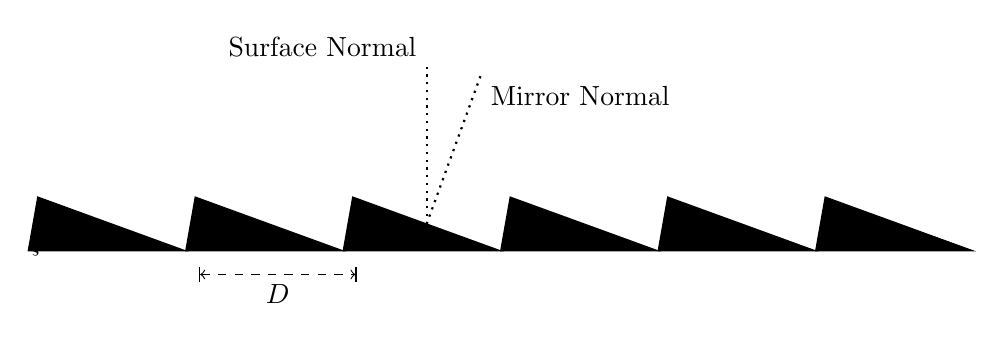
\begin{tikzpicture}
            \foreach \x in {0, 2, ..., 10} {
                \draw[fill=black] (\x, 0) -- (\x + 2, 0) -- ++(160:2) -- cycle;
            }

            \draw[thick, dotted]
            ({6 - cos{20}}, {sin(20)})
            -- ++(90:2) node[above left] {Surface Normal};

            \draw[thick, dotted]
            ({6 - cos(20)}, {sin(20)})
            -- ++(70:2) node[below right] {Mirror Normal};

            \centerarc[->]({6 - cos(20)}, {sin(20)})(90:70:1.8)
            node[midway, above] {$\xi$};

            \draw[|<->|, dashed] (2, -.3) -- (4, -.3) node[midway, below] {$D$};
        \end{tikzpicture}

        \caption[Blazed Grating]{
            The surface of a blazed reflection grating.
            The blaze angle is $\xi$.
        }
        \label{fig:blazed-grating}
    \end{figure}

    This improvement throws a \textbf{blaze} of light into a particular order.
    Such a grating is therefore called a \textbf{blazed diffraction grating}.
    The blaze angle does not affect the sine-squared ratio that produces the part of the diffraction pattern that gives you sharp spots of light, because that part depends only on the spacing between elements of the geometry.
    The blaze angle also does not affect Equation~\eqref{eqn:non-normal-grating-equation} because $\theta_i$ and $\theta$ are measured from the surface normal.
    It only affects the amount of power going into each order.

    To make effective use of a blazed diffraction grating, we need to build an optical device around the grating.
    One design is the \textbf{Ebert-Fastie grating spectrometer}, shown in Figure~\ref{fig:ebert-fastie}.
    It is designed to be used with a blazed diffraction grating, with the blaze angle $\xi$ chose to be approximately equal to $\alpha_0$, and the diffraction grating placed at the focal point of a concave mirror.
    This sends the blaze of light through the exit slit.

    \begin{figure}[H]
        \centering

        \begin{tikzpicture}[scale=0.9]
            % entrance slit
            \draw[very thick] (-1, 2) -- (-1, 2.9);
            \draw[very thick] (-1, 3.1) -- (-1, 4) node[above, right] {Entrance Slit};

            % exit slit
            \draw[very thick] (-1, -2) -- (-1, -2.9);
            \draw[very thick] (-1, -3.1) -- (-1, -4) node[below, right] {Exit Slit};

            % light path
            \draw[postaction={on each segment={midarrow={stealth}}}]
            (-1.5, 3)
            -- (8, 3)
            -- (0, 0)
            -- (8, -3)
            -- (-1.5, -3);

            % mirror
            \pgfmathsetmacro{\r}{sqrt(8*8 + 3*3)};
            \centerarc[very thick](0, 0)(-30:30:\r) node[left] {Concave Mirror};

            % grating
            \draw[fill, rotate around={-10:(0, 0)}] (-.25, -1) rectangle (0, 1);
            \node[left] at (-.25, 0) {Diffraction Grating};

            % grating angle
            \draw[dashed] (0, 0) -- (-100:2);
            \draw[dashed] (0, 0) -- (-90:2);
            \centerarc[<->, very thick](0, 0)(-90:-100:1.8) node[midway, below] {$\beta$};

            \draw[dashed] (0, 0) -- (-10:3);
            \centerarc[<->](0, 0)(20.5:-10:2) node[midway, right] {$\theta_i$};
            \centerarc[<->](0, 0)(-10:-20.5:2.8) node[midway, right] {$-\theta$};

            \draw[dashed] (0, 0) -- (0:\r);

            \centerarc[<->](0, 0)(20.5:0:5) node[midway, right] {$\alpha$};
            \centerarc[<->](0, 0)(0:-20.5:5) node[midway, right] {$\alpha$};
        \end{tikzpicture}

        \caption[Ebert-Fastie Spectrometer]{The optical path of an Ebert-Fastie grating spectrometer.}

        \label{fig:ebert-fastie}
    \end{figure}

    \newpage
    \section*{Equipment}

    For this lab, you will need:
    \begin{itemize}
        \item The two calibration lasers (\SI{405}{\nano\meter} and \SI{635}{\nano\meter}), with mounts.
        \item A sodium vapor lamp.
        \item A lamp with an unidentified element in it.
        \item A hydrogen lamp.
        \item An Ebert-Fastie grating spectrometer.
        \item A photomultiplier tube (PMT).
        \item An electrometer.
    \end{itemize}
    \noindent
    The photomultiplier tube uses high-voltage plates to convert a small flux of photoelectrons from the interferometer into a measurable current.
    The photomultiplier requires a negative voltage to operate.
    \textbf{Do not exceed 600 volts on the photomultiplier!}


    \FloatBarrier
    \newpage

    \section*{Procedure}

    \subsection{Calibrating the Spectrometer}

    To calibrate the spectrometer, you need to find two points on the micrometer  where you know the wavelength of the light passing through the exit slit.
    Based on the position of the grating at these two points, you can determine how the position of the grating maps to differences in wavelengths.
    
    A convenient source of known-wavelength light is a laser, and you've been provided two lasers: one has a wavelength of \SI{532}{\nano\meter} and the other has a wavelength of \SI{635}{\nano\meter}.  Shine each laser through the entrance slit so that the reflection off of the first mirror hits the grating in the middle.  
    Do this for every light source. 
    Since the grating is at the focal point of the two mirrors, this will ensure that the light arrives at the exit slit  at a consistent angle.  Slowly move the micrometer over a wide range until you see a spike on the electrometer.  This position on the micrometer then corresponds to the wavelength of the laser you are using.

    \checkpoint{
        Calibrate your spectrometer using the two lasers.
        \begin{itemize}
            \item What's the last digit that you can reliably read off of the micrometer?
            This is a good rough estimate of the uncertainty in your position measurements.
            \item What is the ratio of your uncertainty to the total distance you moved the micrometer during your calibration measurement?
            This is a good estimate of the fractional uncertainty in your calibration.
            \item How do you convert from the micrometer reading to wavelength?
        \end{itemize}
    }

    \subsection{Measuring the Spectrum of Sodium}

    Hot sodium vapor emits light at around \SI{589}{\nano\meter}.

    \checkpoint{
        Measure the emission wavelength of sodium vapor using your spectrometer.
        \begin{itemize}
            \item  Were you able to resolve the two closely-spaced emission lines near \SI{589}{\nano\meter}?
        \end{itemize}
    }

	\subsection{Identifying an Element}
	Every ionization state of every element produces a unique emission spectrum, so therefore the species can be identified by looking at its emission spectrum.
	This method of identification gives rise to the powerful technique of emission spectroscopy.
	
	Turn the unidentified lamp on and shine its light through the entrance slit so that the reflection off of the first mirror hits the grating in middle.  Start with the micrometer at a position corresponding to 700 nm and slowly move it down to 400 nm.  Record each wavelength that causes the electrometer to spike.

	\begin{table}[H]
		\centering
		\begin{tabular}{c|c|c|c}
			Helium I & Carbon I & Magnesium I & Mercury I \\
			\hline
			447.1 & 538.0 & 426.7 & 404.6 \\
			501.6 & 601.3 & 435   & 407.8 \\
			587.6 &       & 457   & 435.8 \\
			667.8 &       & 517   & 546.1 \\
                  &       & 518   & 577.0 \\
                  &       & 571   & 579.1 \\
                  &       &       & 690.7
		\end{tabular}
		\caption{
            The wavelengths of the emission spectra for four un-ionized elements, in nanometers.
		    This table only shows the strongest lines between \SI{400}{\nano\meter} and \SI{700}{\nano\meter}.
        }
		\label{table:emission-spectra}
	\end{table}

	\checkpoint{
	Measure the emission spectrum of the unidentified element using your spectrometer.
	\begin{itemize}
		\item Use your spectrum and Table \ref{table:emission-spectra} to identify the element in the lamp.
	\end{itemize}
	}

    \subsection{Measuring the Rydberg Constant}

    Spectrometers can also be used to measure constants related to quantum mechanics.
    Since the atoms producing the spectra can be described by quantum mechanics, the spacing of the lines in these spectra depend on the quantum nature of the atoms.
    In this lab we'll use it to measure the \textbf{Rydberg constant}.
    As a reminder, the \textbf{Rydberg formula} for the wavelength of the electronic transitions in hydrogen is
    \begin{align}
        \frac{1}{\lambda} = R_{\infty} \abs{\frac{1}{n_f^2}-\frac{1}{n_i^2}},
    \end{align}
    where $\lambda$ is the wavelength of light emitted from the transition, $R_{\infty}$ is the Rydberg constant, $n_f$ is the principal quantum number of the final state of the electron, and $n_i$ is the principal quantum number of the initial state of the electron.

    For historical reasons, transitions that can be described by the Rydberg formula are grouped into ``series'' by their final state.
    For example, transitions to the hydrogen $n_f=1$ level are called the Lyman series, the $n_f=2$ transitions are the Balmer series, the $n_f=3$ transitions are the Paschen series, etc.
    The lowest energy transition in a series is known as the $\alpha$ line, the second-lowest as the $\beta$ line, and so forth.

    \checkpoint{
        Measure the wavelengths of the Balmer $\alpha$ ($n_i = 3$, $n_f = 2$, $\lambda = \SI{656}{\nano\meter}$) and Balmer $\beta$ ($n_i = 4$, $n_f = 2$, $\lambda = \SI{486}{\nano\meter}$) emission lines of hydrogen and use them to calculate the Rydberg constant $R_{\infty}$.
        Compare your measurement to the expected value ($R_{\infty} = \SI{109737.3}{\per\centi\meter}$).
    }

    \FloatBarrier
    \newpage

    \section*{Prelab Questions}
    \setcounter{subsection}{0}

    \subsection{Ebert-Fastie Grating Equation}

    Using the angles $\theta_i$, $\theta$, $\alpha$, and $\beta$ that are given in Figures \ref{fig:path-length-difference-non-normal} and \ref{fig:ebert-fastie}, show that the grating equation $D(\sin\theta_i + \sin\theta) = m \lambda$ is equivalent to
    \begin{align*}
        2 D \cos\alpha \sin\beta = m \lambda.
    \end{align*}
    Be careful with the orientation of $\theta$.

    \vspace{\stretch{1}}

    \subsection{Ebert-Fastie Sine Bar}

    Suppose that a \textbf{sine bar} (shown in Figure~\ref{fig:sine-bar}) is used to rotate the grating of an Ebert-Fastie grating spectrometer.
    Show that the wavelength of the light passing through the exit slit changes linearly with the displacement of the sine bar ($x$ in the figure).

    \begin{figure}[H]
        \centering

        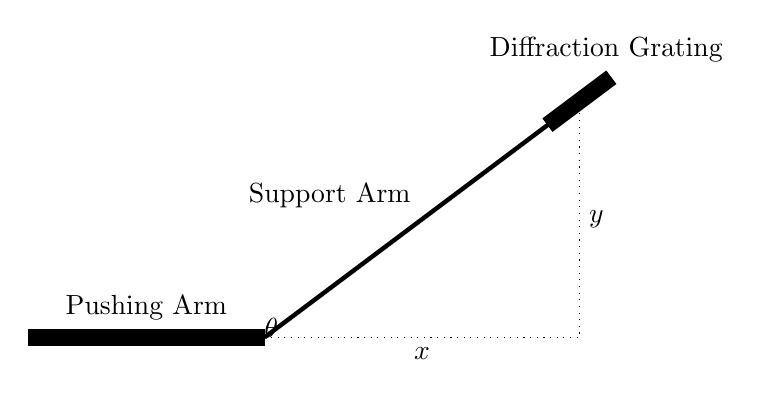
\begin{tikzpicture}
            \draw[ultra thick] (0, 0) -- (4, 3) node[midway, above left] {Support Arm};
            \draw[dotted] (0, 0) -- (4, 0) node[midway, below] {$x$} -- (4, 3) node[midway, right] {$y$};

            \draw[fill=black, rotate around={36.87:(4, 3)}] (3.50, 2.90) rectangle ++(1, .2) node[above] {Diffraction Grating};

            \draw[fill=black] (-3, -.1) rectangle ++(3, .2) node[midway, above, yshift=.1cm] {Pushing Arm};

            \centerarc[<->](4, 3)(-91:{-90-53.13+1}:2) node[midway, above] {$\theta$};
        \end{tikzpicture}

        \caption[Sine Bar Mechanism]{
            A sine bar.
            The pushing arm (typically a micrometer) changes the displacement $x$.
            The resting position is $x=0$.
            The contact point between the pushing arm and the support arm is allowed to slip slightly as the arms are moved so that the path is straight instead of curved (the distances drawn in the figure are exaggerated compared to a real sine bar).
        }

        \label{fig:sine-bar}
    \end{figure}

    \vspace{\stretch{2}}

\end{document}
